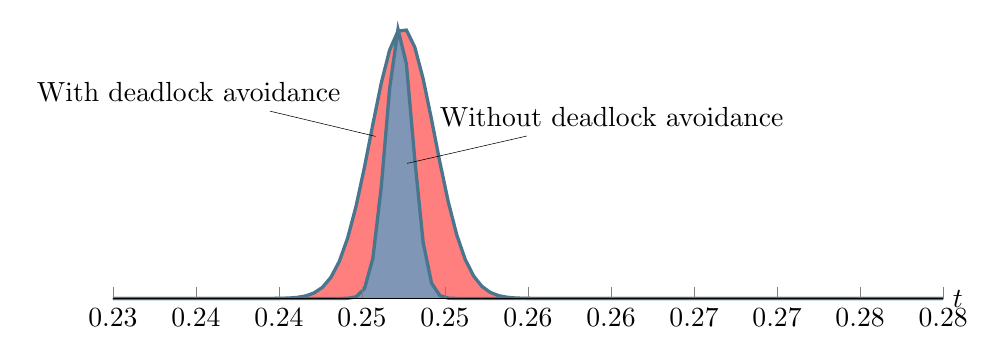
\begin{tikzpicture}
\begin{axis}[
  no markers, domain=0.230:0.280, samples=100,
  axis lines*=left, xlabel=$t$, ylabel=$1$,
  hide y axis,
  every axis x label/.style={at=(current axis.right of origin),anchor=west},
  height=5cm, width=\linewidth,
  ytick=\empty,
  %xtick={0.253917}, ytick=\empty,
  enlargelimits=false, clip=false, axis on top,
  %grid = major % Will draw full horizontal lines
  ]
  
  % Base sample (pthreads only)
  % Mean=0.247245 s, stdiv=0.000812878 s, normalized PDF=E^(-756693. (-0.247245+x)^2)
  
  % Experimental sample (deadlock resolution)
  % Mean=0.247453 s, stdiv=0.00191479 s, normalized PDF=208.348 E^(-136373. (-0.247453+x)^2)
  
  \addplot [very thick,cyan!50!black, fill=red, fill opacity=0.5] {e^(-136373 * (-0.247453+x)^2};
  
  \addplot [very thick,cyan!50!black, fill=cyan, fill opacity=0.5] {e^(-756693 * (-0.247245+x)^2};
  
  \node [
	  coordinate,
	  pin={[pin edge={black}]135:{With deadlock avoidance}},
	  style={xshift=-0.3cm}
  ] 
  at (axis cs:0.247245,0.6) {};
  
  \node [
	  coordinate,
	  pin={[pin edge={black}]50:{Without deadlock avoidance}},
	  style={xshift=0.1cm}
  ] 
  at (axis cs:0.247245,0.5) {};
  
   % [pos=0.5,pin={\color{black}$\mu_1=0.247400\ s$}] {};
   
  
  % [pos=0.5,pin={\color{black}$\mu_0=0.253917\ s$}] {};
  %\addplot [very thick,black, domain=0.25065033:0.25718367]{0.5} node [pos=0.5,label=$\sigma_0\approx 0.003\ s$, style={yshift=-1cm}] {};
\end{axis}
\end{tikzpicture}